\documentclass[onecolumn,draftcls]{IEEEtran}
\usepackage{epsf,graphicx,color,epstopdf}
\usepackage{lineno}
\usepackage{setspace}
\usepackage{hyperref}
\usepackage{soul}

\newcommand{\exvivo}{\textit{ex vivo }}
\newcommand{\invivo}{\textit{in vivo }}
\newcommand{\invitro}{\textit{in vitro }}
\newcommand{\insitu}{\textit{in situ }}
\newcommand{\degree}{$^\circ$}
\newcommand{\isppa}{$I_\textrm{sppa}$}
\newcommand{\etal}{\textit{et al. }}
\newcommand{\attenunit}{dB$\cdot$cm$^{-1}$MHz$^{-1}$}

\title{Acoustic Radiation Force Impulse (ARFI) Imaging Prostate Zonal Anatomy:
    Comparison with Endorectal T2-Weighted MR Imaging (T2WI)}

\author{
    \IEEEauthorblockN{
        (Mark L. Palmeri, M.D., Ph.D.\IEEEauthorrefmark{1}, 
        Kirema Garcia-Reyes\IEEEauthorrefmark{2}), 
        Stephen J.  Rosenzweig\IEEEauthorrefmark{1}, 
        Rajan Gupta, M.D.\IEEEauthorrefmark{3}, 
        Christopher Kauffman, M.D.\IEEEauthorrefmark{3}, 
        Thomas Polascik, M.D.\IEEEauthorrefmark{4},
        Samantha L. Lipman\IEEEauthorrefmark{1},
        Zachary A. Miller\IEEEauthorrefmark{1}, 
        Tyler Glass\IEEEauthorrefmark{1}, 
        Kathryn R. Nightingale, Ph.D.\IEEEauthorrefmark{1}}

    \IEEEauthorblockN{
        {\IEEEauthorrefmark{1}Department of Biomedical Engineering, Pratt School of Engineering, Duke University}
        {\IEEEauthorrefmark{2}Duke University School of Medicine}
        {\IEEEauthorrefmark{3}Department of Radiology, Duke University Medical Center}
        {\IEEEauthorrefmark{4}Department of Surgery (Urology), Duke University Medical Center}
        {\IEEEauthorrefmark{5}Department of Pathology, Duke University Medical Center}
    }
}


\begin{document}

\maketitle

\linenumbers

\section*{Abstract}
Prostate cancer (PCa) is the most common non-cutaneous malignancy among men in
the United States and the second leading cause of cancer related death.
Non-invasive imaging could lead to improved diagnosis, risk-stratification, and
PCa management.  Magnetic resonance imaging (MRI) has been available for use in
the workup of patients with PCa since the early 1980s, and recent advances with
functional parameters has greatly improved its clinical diagnostic utility.
Acoustic Radiation Force Impulse (ARFI) imaging is an ultrasound-based modality
that evaluates the mechanical properties of soft tissues. ARFI imaging has the
potential to aid in PCa diagnosis and management by evaluating the structural
composition of prostate zones and tumors based on their stiffness.  In this
study, MR and ARFI imaging datasets were compared to one another and with gross
pathology measurements made immediately post radical prostatectomy.  Imaging
datasets were manually segmented to delineate the central gland and prostate
capsule, and 3D models were rendered to evaluate zonal anatomy dimensions and
volumes.  Both imaging modalities showed moderate correlations (0.39 $<$ R$^2 <
$ 0.74) between estimated organ volume and gross pathologic weights.  ARFI and MR
total prostate gland volumes were well-correlated (R$^2$ = 0.68), but ARFI
images yielded prostate volumes that were, on average, larger (36\% $\pm$ 28\%)
than MR images, primarily due to over-estimation of the anterior-to-posterior
dimension of the prostate total gland (17.0 $\pm$ 12.1\%), while over-estimates
of the other dimensions were less significant contributors (8.1 $\pm$ 18.4\%
and 0.58 $\pm$ 12.9\%).  The central zone volumes of ARFI and MR images were
also moderately correlated (R$^2$ = 0.41), with minimal volume bias between the
imaging modalities, but significant variability case-to-case (2.1 $\pm$
39.1\%).  Central zone volume differences were, again, strongly attributed to
over-estimation of the anterior-to-posterior axis (14.8 $\pm$ 23.1\%), with a
significant underestimation of the apex-to-base dimension (-10.8 $\pm$ 22.3\%)
and no mean bias in the lateral-to-lateral measurements (0.006 $\pm$ 17.2\%).
Strong variability in central gland volumes is believed to be related to the
extent of benign prostatic hyperplasia (BPH) for select cases.  Overall, ARFI
imaging of the prostate yielded prostate volumes and dimensions that were
correlated with MR T2WI estimates, with biases in the anterior-to-posterior
dimension, most likely related to poor displacement SNR in the anterior region
of the prostate from greater distance from the rectal wall imaging surface.
ARFI imaging is a promising low-cost, real-time imaging modality that can
compliment MR imaging for diagnosis, treatment planning and management of PCa.


\section{Introduction}\label{sect:intro}

\begin{itemize}
	\item Motivation!!
	\item Paper outline
\end{itemize}


Clinical Background and Significance 
Prostate cancer (PCa) is the most common noncutaneous malignancy among men in the United States. Approximately 1 in every 6 men will develop PCa during their lifetime, with the median age of diagnosis at 67. i It is also the second leading cause of cancer related death, with 1 in 36 men dying from the disease. The National Cancer Institute estimates that 238,590 men will be diagnosed with PCa in 2013 and 29,720 will die from the disease.ii

PCa diagnosis usually begins by screening with prostate specific antigen (PSA) and digital rectal examination (DRE).  Definitive diagnosis is made by random ultrasonography-guided transrectal (TRUS) biopsies, which are then used to provide the clinician with the proper Gleason score. The combination of these factors—as well as staging—determines the appropriate therapy and prognosis. 

PCa screening has led to earlier diagnosis of smaller tumors and more localized disease.  However, it is well known that the sensitivity and specificity of PSA and DRE are not optimal. In addition, DRE has a low predictive value at lower PSA ranges, and PSA yields many false positives. .iii iv  As such, a theoretical risk of over-diagnosis and treatment of low-grade—and possibly clinically insignificant—disease exists. Moreover, due to the random nature of biopsies, cancer located outside the routine sampling site can be missed and the extent of the cancer might be underestimated.v vi For example, in a study by Mufarrij et al 45.9%-47.2% of patients who were candidates for active surveillance but underwent radical prostatectomy had a higher Gleason score on final histopathology than after TRUS biopsy.vii These inaccuracies may lead to inappropriate diagnosis, imprecise risk assessment and potentially avoidable morbidity.

The Use of Magnetic Resonance Imaging in Prostate Diagnostics
Magnetic resonance (MR) imaging has been available for use in the workup of patients with PCa since the early 1980s but the early work on its diagnostic accuracy is heterogeneous. viii Earlier MR techniques relied mostly on morphology via T1 and T2- weighted imaging (T2WI). The more recent ability to include not only anatomic but also biologic and functional dynamic parameters into MR analysis—via diffusion-weighted imaging (DWI), dynamic contrast-enhanced (DCE) imaging or MR spectroscopic imaging (MRSI)—is promising in the future diagnosis and management of PCA.

 Currently prostate MR focuses on a multiparametric approach, where 2 or more imaging sequences—including anatomic and functional data—are used together to try to arrive to a diagnosis.ix As MR technology continues to evolve and improve, its role in PCA diagnosis, staging, treatment planning and follow-up has gained much attention.

 T2-Weighted Imaging
 T2WI sequences are crucial components of prostate MR imaging.  T2WI is particularly useful in prostate analysis due to its excellent soft tissue contrast resolution, which can be maximized by using thin sections of 3-4mm and a small field of view of approximately 14cm. x xi xii T2 sequences are the most helpful for tumor localization as they can clearly show overall prostate morphology, internal structures and prostatic margins.xiii Seventy five percent of prostatic tumors are found in the peripheral zone (PZ) and normally show hypointense T2 signal when compared to the higher intensity PZ.xiv xvHowever tumors can sometimes seem of similar intensity as the surrounding tissue and false positives can occur secondary to post biopsy changes/hemorrhage, hyperplasia or prostatitis, making diagnosis more challenging.xvi 

 Functional MR Sequences
 Even though T2WI is the mainstay of prostate MR, its overall performance in prostate cancer diagnosis is not optimal. The incorporation of two or more functional sequences in multiparametric MR imaging (mpMRI) has been shown to significantly improve the performance of MR in cancer diagnosis.xvii In fact, the European Society of Urogenital Radiology’s (ESUR) prostate MR guidelines recommend at least 2 functional imaging techniques in addition to T2WI in order to better characterize prostate tumors.xviii  In a study by Turkbey et al, researchers found that mpMRI had a positive predictive value of 98% in prostate cancer detection.xix These functional sequences include diffusion- weighted imaging (DWI), dynamic contrast enhanced imaging (DCE-MRI) and MR spectroscopic imaging (MRSI). 

 Diffusion-weighted imaging
 DWI is based on the free movement of water particles in tissue and measures the degree of motion restriction.xx Normal prostatic tissue is very glandular with plenty of water molecule movement. On the other hand tumors have high cellular density and restricted water movement, which leads to decreased diffusion. Due to this restricted diffusion, tumors seem to be of higher intensity on DWI.xxi 

 DWI sequences can be processed to obtain apparent diffusion coefficient (ADC) maps. These serve as a more objective measure of diffusivity since they are independent of magnetic field and thus overcome the effects of T2 shine-through.xxii xxiii ADC maps are also used to visually assess the tumor, which appears as a focus of decreased signal intensity when compared to normal prostate tissue.xxiv 

 In addition to knowing the location of the cancer within the prostate, being able to identify which cancers will exhibit more aggressive behavior is important when making clinical management decisions. A number of studies have found that lower ADC values correlate with tumors that have higher Gleason scores. xxv xxvi xxviiThis could be explained by the fact that higher-grade lesions are usually of higher cellular density and thus have even more marked restricted diffusion. This inverse correlation suggests that ADC maps might be helpful when characterizing lesions and assessing tumor aggressiveness. xxviii 

 Dynamic contrast enhanced imaging
 DCE-MRI has been shown to have a high sensitivity in cancer detection, especially when combined with other MR imaging modalities.xxix xxx xxxi xxxii In a study by Hara et al, this functional modality identified 93% of clinically significant cancers.xxxiii DCE-MRI provides a measure of tumor vascularity and takes advantage of tumor-induced angiogenesis in PCa. xxxiv Increased vascularity in prostate cancer results in earlier and higher peak contrast enhancement and a faster washout when compared to normal prostatic tissue.xxxv  These known characteristics of PCa are helpful when trying to localize lesions. 

 A variety of different approaches can be used to analyze DCE-MRI and no report has, up to date, described the superiority of one method over the others.xxxvi The approaches include qualitative analysis by visual assessment of the images, semi-quantitative methods that look at kinetic parameters on a voxel-by-voxel basis, or quantitative methods that that convert signal intensity into kinetic parameters to determine how much contrast is being exchanged between the vascular, extravascular and extracellular spaces.xxxvii 
    
    MR spectroscopy
    Like DWI, MRSI can be helpful in lesion characterization as it provides information on the presence of certain metabolites in tissue. xxxviii Choline and citrate are especially useful in the setting of PCa. Choline is critical in cell membrane synthesis and is thus usually elevated in cells with cancerous behavior.xxxix Healthy prostate epithelium synthesizes and secretes large quantities of citrate but levels are decreased in PCa.xl xliTherefore, an increase in the choline-to-citrate ratio on MRSI can be used as an indicator of malignancy.xlii 

    Although some data suggests that MRSI increases the accuracy of tumor volume detection and staging when used in addition to anatomic imaging, it is unclear whether it is superior to other modalities.xliii ESUR lists MSRI as an optional modality for the diagnosis of PCa since it significantly lengthens exam time and requires specific technical expertise.xliv Many academic centers in the United States do not include MSRI in their mpMRI prostate cancer protocols.xlv 


\section{METHODS}\label{sect:methods}

\subsection{Study Inclusion Criteria}
Patients undergoing radical prostatectomy for biopsy-proven PCa treatment were
enrolled as study subjects in this IRB-approved (Duke IRB\# Pro00006458),
HIPAA-compliant study.  A total of 16 patients were recruited and enrolled in
this study.  Inclusion criteria were undergoing complete pelvic MRI with
endorectal coil for detection of prostate cancer, including multiplanar
T2-weighted anatomic imaging, as well as pre-operative ARFI imaging and radical
prostatectomy.  Patients with previous treatments of PCa or benign prostatic
hyperplasia (BPH), or anatomic anomalies of the rectum, were excluded from this
study.  All patients enrolled in this study provided written informed consent.

\emph{CO-AUTHOR QUESTION: DO WE WANT TO INCLUDE A TABLE OF PATIENT DEMOGRAPHIC INFORMATION?}


\subsection{Pathology Processing}
After excision, the prostates were weighed and tri-axially measured, formalin
fixed for at least 24 hours without being cut, and then processed for whole
mount histology.  While tri-axial measurements of the gross prostate were not necessarily anatomically aligned, rough estimates of the prostate volume were made using a tri-axial, ellipsoidal organ volume assumption, where the volume could be estimated as:

\begin{equation}
V = \frac{4}{3}\pi \sqrt{\det{A^{-1}}},
\end{equation}

where $A$ represents the eigenvector matrix of the tri-axial pathology
measurements.



\subsection{MR Imaging}
All MR imaging was performed on one of two 3.0 Tesla MR scanners (General
Electric HDx, GE Healthcare, Waukesha, WI;  Siemens Skyra, Siemens Healthcare,
Erlangan, Germany) using a single channel Medrad eCoil endorectal coil (Medrad,
Indianola, PA), as well as multi-channel surface coils.  Imaging sequences
included thin-section (3 mm section thickness) fast spin echo T2-weighted
images in the coronal, axial and sagittal planes.  Diffusion weighted images
(DWI) were obtained using multiple b-values and calculation of Apparent
Diffusion Coefficient (ADC) maps was also performed.  Dynamic contrast enhanced
MR (DCE-MRI) sequences were obtained after administration of a weight-based
dose of extracellular MR contrast agent \textbf{(Magenvist\textregistered,
Bayer Pharma AG)} with 4-5 second temporal resolution for 5-6 minutes.
\textbf{While the DWI and DCE-MRI images were used in conjuntion with the T2W
images for lesion characterization, the DWI and DCE-MRI images were lower
resolution and do not add much information to the T2W images for the purposes
of delineating prostate size and segmentation.
}


\subsection{ARFI Imaging}
Experimental ARFI imaging data were acquired using a modified Siemens Acuson
SC2000\texttrademark~ultrasound scanner (Siemens Healthcare, Ultrasound Business Unit,
Mountain View, CA, USA) and the longitudinal array of an Acuson ER7B
transducer.  The ARFI imaging sequence was comprised of
standard B-mode ultrasonic imaging, or tracking beams, and pushing beams. For
each lateral location, two pre-push reference images were acquired, then three
300 cycle pushing pulses were transmitted in rapid succession, focused at 30
mm, 22.5 mm, and 15 mm, respectively, and finally the response of the tissue
was tracked for up to 6ms at a PRF of 8kHz. This pushing strategy is similar to
what has been published by Bercoff \etal~\cite{Bercoff2004}. The 30 mm and 22.5
mm foci pushing pulses were transmitted at 4.6 MHz with a F/2 geometry and the
15 mm focus pushing pulse was transmitted at 5.4 MHz with a F/2.35 geometry to
maintain the same beamwidth (0.67 mm) throughout the region of excitation. A
total of 82 lateral locations were interrogated to cover the 55 mm field of
view, translating 0.67 mm laterally per location.

For the tracking pulses, 16 parallel receive lines at 5.0 MHz were spaced to
observe both the on and off-axis response of the tissue to the pushing pulses.
Specifically, four lines were dedicated to tracking the on-axis displacement,
with all 4 beams located inside the beamwidth of the pushing pulses such that
the beam spacing was 0.17 mm. 

3D volumetric imaging data was acquired using mechanical rotation of the ER7B
transducer between sequential imaging frames, sweeping across the lateral
extent of the prostate.  This rotation setup utilized a CIVCO
Micro-Touch\texttrademark stabalizer (CIVCO Medical Solutions, Kalona, IA USA)
that allows for complete 6-axis degrees of freedom for manual positioning of
the transducer to sweep through the entire prostate during imaging.  Sequential
imaging frames were $\sim$1\degree apart, depending on the absolute size of the
prostate.  A custom optical angular feedback transduction circuit utilizing a
reflective linear strip with 500 lines-per-inch (LPI) resolution (US Digital,
Vancouver, WA, USA) was coupled with a 141 oz-in torque stepper motor with
planetary gearbox (Model \#11YPG202S-LW4-R27, Anaheim Automation, Anaheim, CA,
USA) (Figure~\ref{fig:setup_annotated}) to achieve accurate spatial
localization of the imaging frames in the 3D dataset.

\begin{figure}[htb!]
\centering
\includegraphics[width=0.75\textwidth]{figs/setup_annotated.png}
\caption{The experimental setup used for ARFI imaging in the operating suite,
    including the Siemens SC2000 scanner with the ER7B endorectal transducer
    sitting in a custom cradle of a CIVCO Micro-Touch\texttrademark stabalizer
    with optical feedback controlling a stepper motor to acquire 3D ultrasound
    imaging data \invivo.  Custom-written Python code was run on the scanner to
    trigger B-mode and ARFI imaging acquisition sequences relative to completed
    rotation increments of $\sim$ 1-2\degree.}
\label{fig:setup_annotated} 
\end{figure}


Displacement estimation was performed using a phase-shift estimator on the
beamformed in-phase and quadrature (IQ) data~\cite{Loupas95,pinton06}. The ARFI
data were then normalized as a function of depth to account for attenuation and
focal gain effects.  This normalization was performed using a displacement
profile measured in a homogeneous tissue-mimicking phantom, which was applied
to all displacements in the entire data set at each time step, and then
low-pass filtered with a cutoff-frequency of 0.8 mm$^{-1}$.

The normalized displacement data were scan-converted using a Delaunay
triangulation method with XXXX commaind in Matlab (R2012b, XXXX).  The
scan-converted ARFI imaging data had a final voxel size of XX x XX x XX mm.


\subsection{Image Zonal Anatomy Segmentation and 3D Model Rendering}
Axial T2W MR slices were manually segmented using the polygon tool on
ITK-SNAP~\cite{Yushkevich2006} using separate labels for the peripheral zone
(PZ), central gland (CG) and anterior fibromuscular stroma (AFS). The gland was
segmented from base to apex.  The base was identified below the bladder and
subsequent images were segmented until the last slice with visible prostatic
tissue was identified caudally. The CG, PZ and AFS were segmented independently
according to their well-established anatomical characteristics on
T2WI.~\cite{Verma2011,Jung2012,Poon1985,Hricak2007,Bonekamp2011} The PZ was
identified by its homogenous high signal intensity on T2WI, which is usually
similar to that of the nearby periprostatic fat. The CG was visualized and
delineated based on its heterogeneous and lower signal intensity as well as its
location. Although not readily visible on every case, the AFS was identified by
its low T2 signal intensity and its location anterior to the central gland. 

ARFI images were segmented using a similar procedure to the MR images, using
XXXX (INSERT CRITERIA HERE).  

Segmented image stacks were imported into 3D Slicer (v4.3.0, CITATION) and 3D
models were rendered using the following parameters (Table~\ref{tab:3dslicer}:

\begin{table}[htb!]
\centering
\caption{3D model volume rendering parameters}
\begin{tabular}{ll}
{\bf Parameter} & {\bf Value} \\ \hline
Decimation & 0.1 \\
Smoothing Algorithm & Laplacian \\
Smoothing  & 70.0 \\
Joint Smoothing & Enabled \\
\end{tabular}
\end{table}



\section{Results}\label{sect:results}
The subvolumes associated with the zonal anatomy in each imaging modality were
measured (Figure~\ref{fig:mr_arfi_volumes}(a)), with moderate correlation
between the ARFI and MR total prostate gland volumes (R$^2$ = 0.63), with a
mean overestimation of of 6.1 $\pm$ 25.0\% by ARFI imaging compared to MR
volumes (Figure~\ref{fig:mr_arfi_volumes}(b)).  Central gland volumes were
slightly less correlated between ARFI and MR images (R$^2$ = 0.38) with no
significant mean over/under-estimation (-5.0 $\pm$ 39.5\%), but significant
variability between the cases (Figure~\ref{fig:mr_arfi_volumes}(c)).
Table~\ref{tab:mr_arfi_volumes} has the individually-measured volumes for MR
and ARFI imaging for each study subject.

\begin{figure}[htb!]
\centering
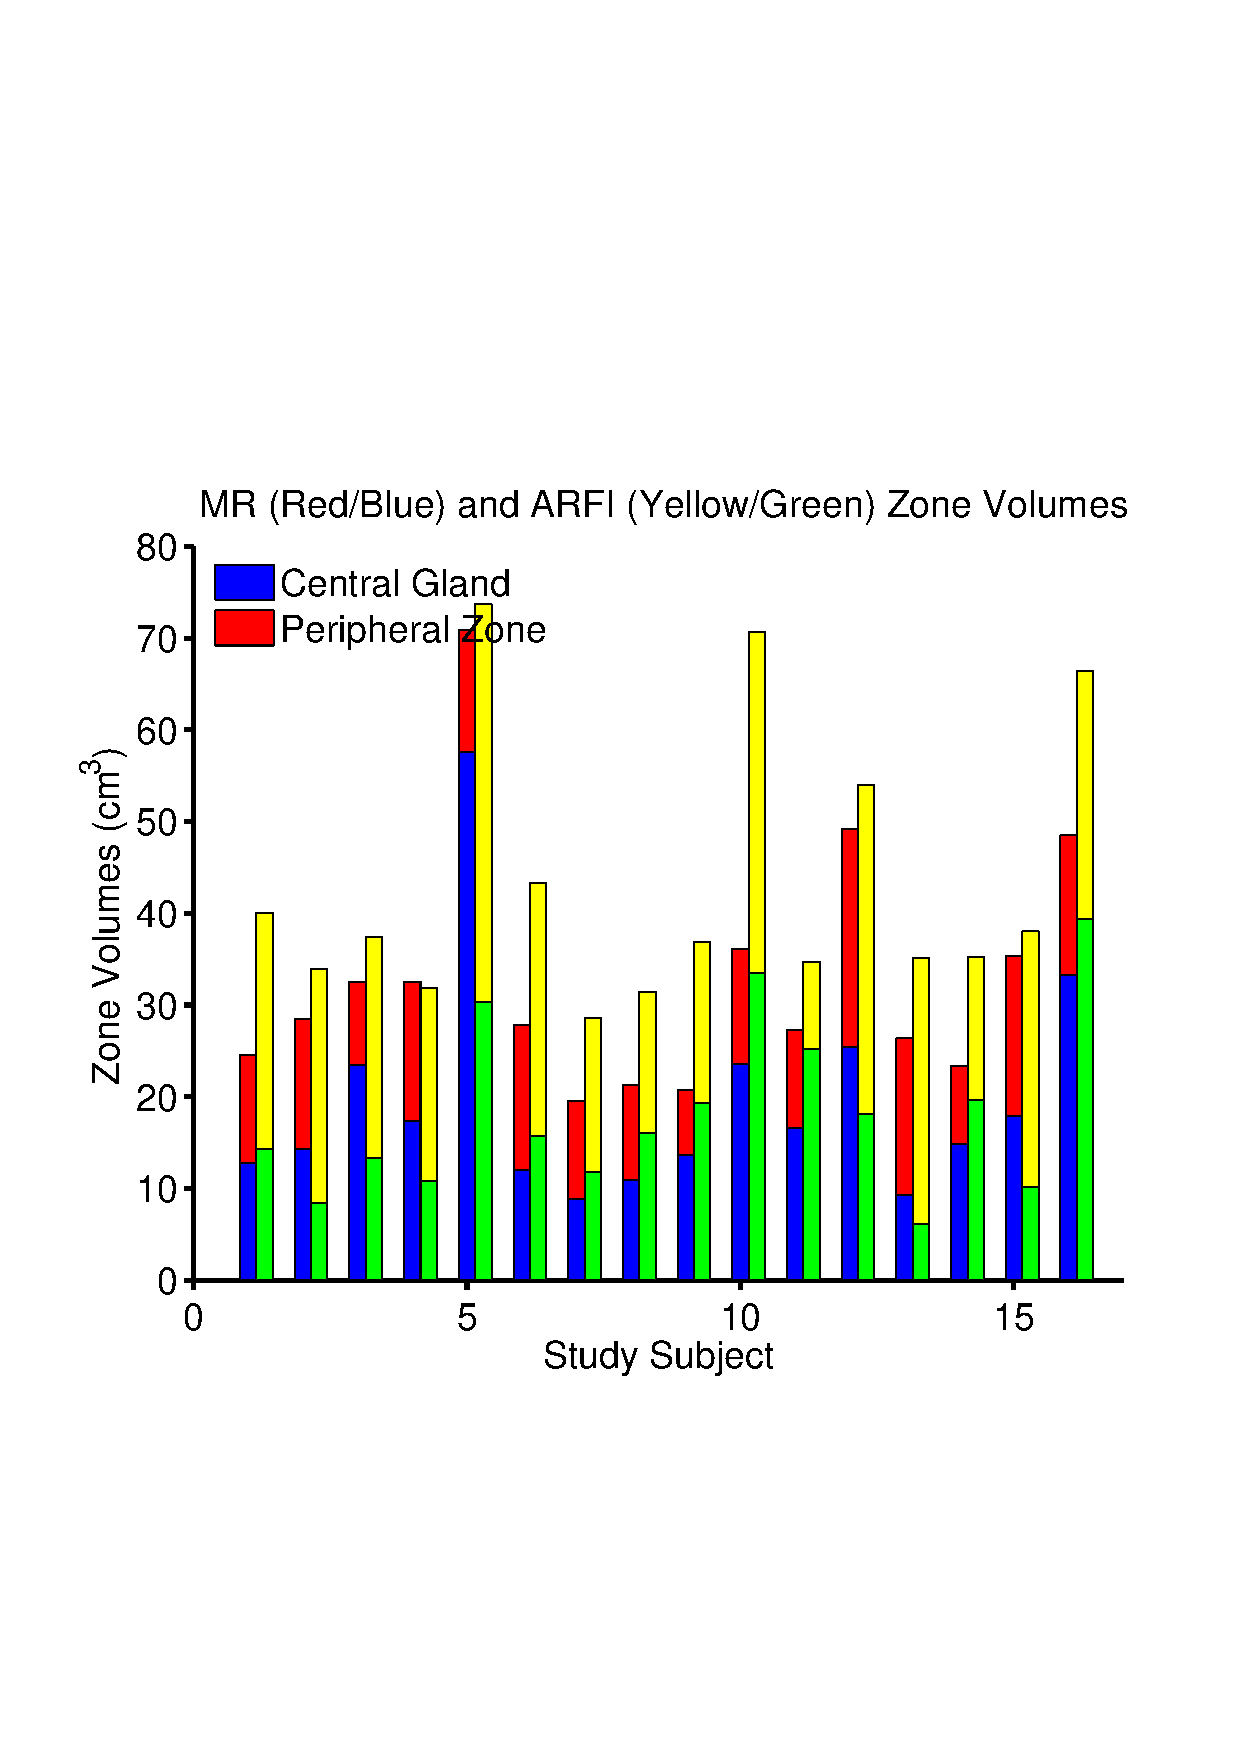
\includegraphics[width=0.5\linewidth]{figs/mr_arfi_volumes.pdf}
\caption{MR and ARFI volumes - need more text here}
\label{fig:mr_arfi_volumes} 
\end{figure}


Weights and axis measurements from the gross pathology processing of the
excised prostates were collected (Table~\ref{tab:path_data}), and using the
axis measurements (lateral-to-lateral, anterior-to-posterior, and
apex-to-base), the prostate volume was approximated as a tri-axial ellipsoid,
and its volume was estimated (\ref{eqn:ellipsoid_volume}).  Prostate weights
were moderately correlated with estimated pathology ellipsoidal prostate
volumes (Figure~\ref{fig:mr_arfi_weight}(a), R$^2$ = 0.68).  There was moderate
correlation between the prostate weight and the image-reconstructed prostate
volumes (Figure~\ref{fig:mr_arfi_weight}(b), R$^2$ = 0.44 (MR) and 0.18
(ARFI)), though there was weaker correlation with the ellipsoidal approximation
of the measurement prostate volume and the image-reconstructed volumes
(Figure~\ref{fig:mr_arfi_weight}(c), R$^2$ = 0.08 (MR) and 0.00 (ARFI)).  

\begin{figure}[htb!]
\centering
\begin{tabular}{lll}
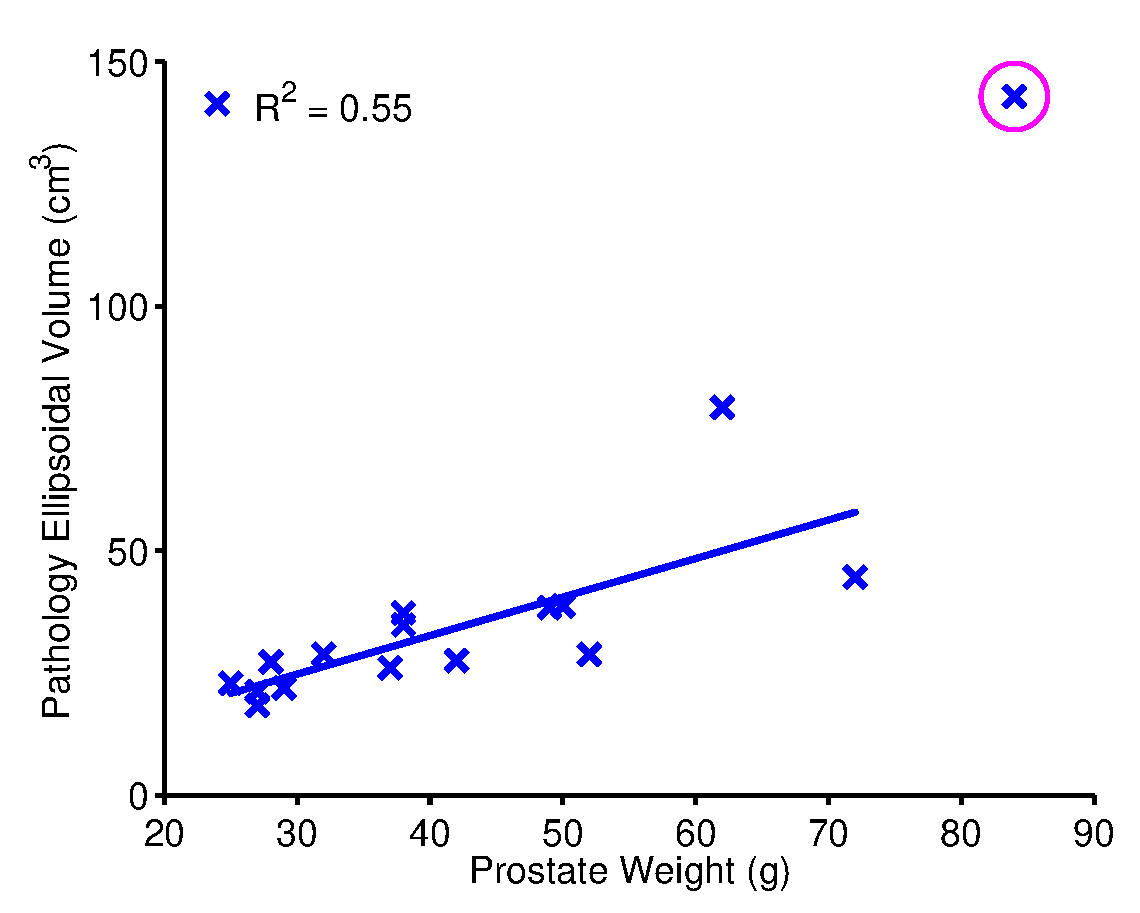
\includegraphics[width=0.3\linewidth]{figs/corr_path_vol_weight_vol} &
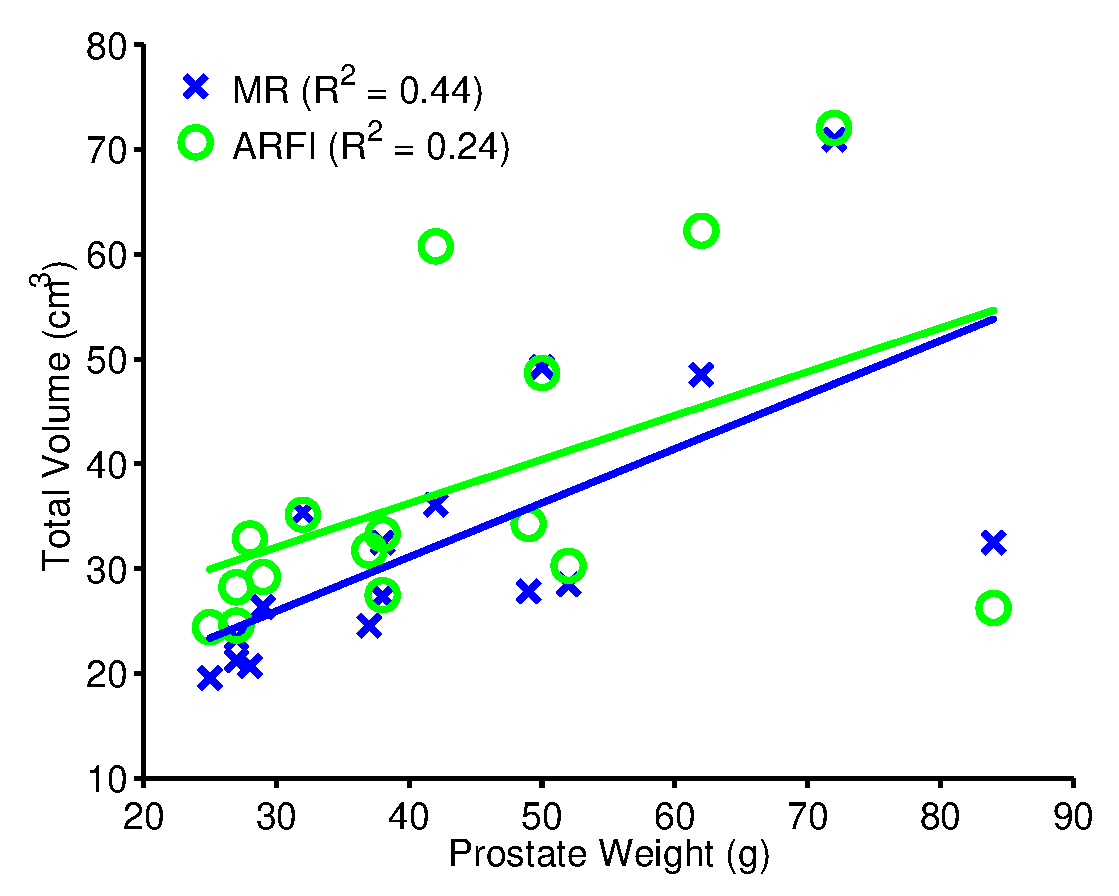
\includegraphics[width=0.3\linewidth]{figs/corr_weight_vol} &
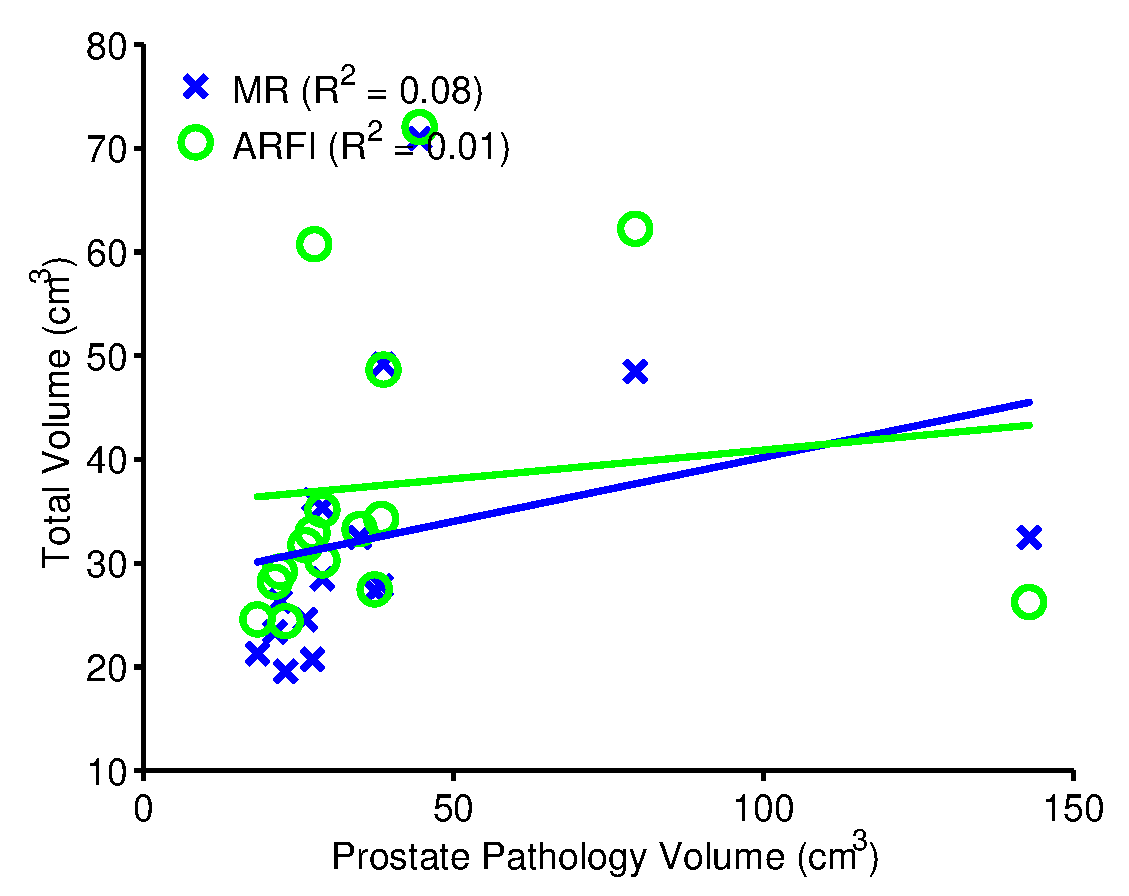
\includegraphics[width=0.3\linewidth]{figs/corr_pathVol_vol} \\
(a) Path Weight : Path Volume & (b) Image Volume : Prostate Weight & (c) Image Volume : Path Volume \\
\end{tabular}
%\begin{tabular}{ll}
%\includegraphics[width=0.3\linewidth]{figs/corr_weight_vol_no4} &
%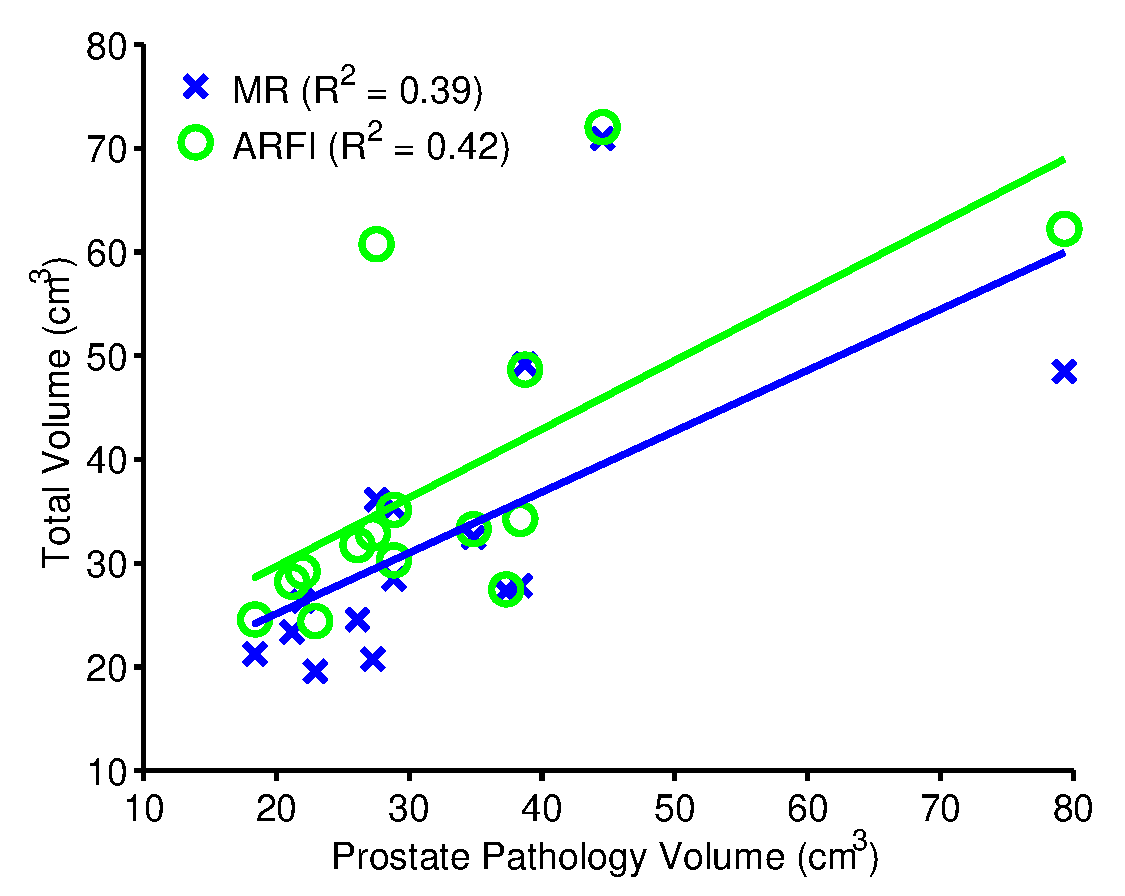
\includegraphics[width=0.3\linewidth]{figs/corr_pathVol_vol_no4} \\
%(d) Image Volume : Prostate Weight (-4) & (e) Image Volume : Path Volume (-4) \\
%\end{tabular}
\caption{Tri-axial pathology measurements were used to make an ellipsoidal
    prostate volume approximation based on gross pathology axis measurements,
    which was moderately well-correlated with the excised prostated weights (a,
    R$^2$ = 0.68).  T2WI MR (blue, X) showed a moderate correlation between the
    reconstructed volumes and prostate weight (R$^2$ = 0.44), while volumes
    reconstructed from ARFI images (green, O) showed weaker correlation (R$^2$
    = 0.21) (b).  Even weaker correlations existed between both T2WI MR and
    ARFI image volumens and approaximated ellipsoidal prostate pathology
    volumes (R$^2$ = 0.08 and 0.01, respectively) (c).  It should be noted in
    these figures that two study subjects had excessively large prostates that
    were difficult to fully capture in imaging (volumes $>$ 60 cm$^3$),
    especially in their anterior region, and they were, therefore, grossly
    underestimated in size.}
\label{fig:mr_arfi_weight}
\end{figure}


Measurements of the prostate total and CG dimensions along the three standard
anatomic axes (apex-to-base, lateral-to-lateral, and anterior-to-posterior)
were made (Table~\ref{tab:mr_arfi_axes}), and the correlation between the
imaging axis measurements was analyzed (Figure~\ref{fig:mr_arfi_path_axes}).
ARFI was most correlated to MR in the lateral-to-lateral axis in both the total
and CG (R$^2$ = \totalLatLatRsq and \centralLatLatRsq, respectively), with mean overestimates of 13.5
$\pm$ 11.0\% and 11.5 $\pm$ 22.5\%, respectively
(Table~\ref{tab:mr_arfi_axes_error}).  ARFI had moderate correlation with the
total prostate gland and CG axes in the anterior-to-posterior dimension (R$^2$
= \totalAntPostRsq and \centralAntPostRsq), respectively, with overestimates of 5.7 $\pm$ 20.6
and -6.1 $\pm$ 21.1\%.  ARFI imaging had weak correlation with MR images in the
apex-to-base dimension (R$^2$ = \totalApexBaseRsq, total gland and R$^2$ = \centralApexBaseRsq, central gland), with
differences of 2.4 $\pm$ 17.0 and 1.2 $\pm$ 19.8\%, respectively.

\begin{figure}[htb!]
\centering
\begin{tabular}{ccc}
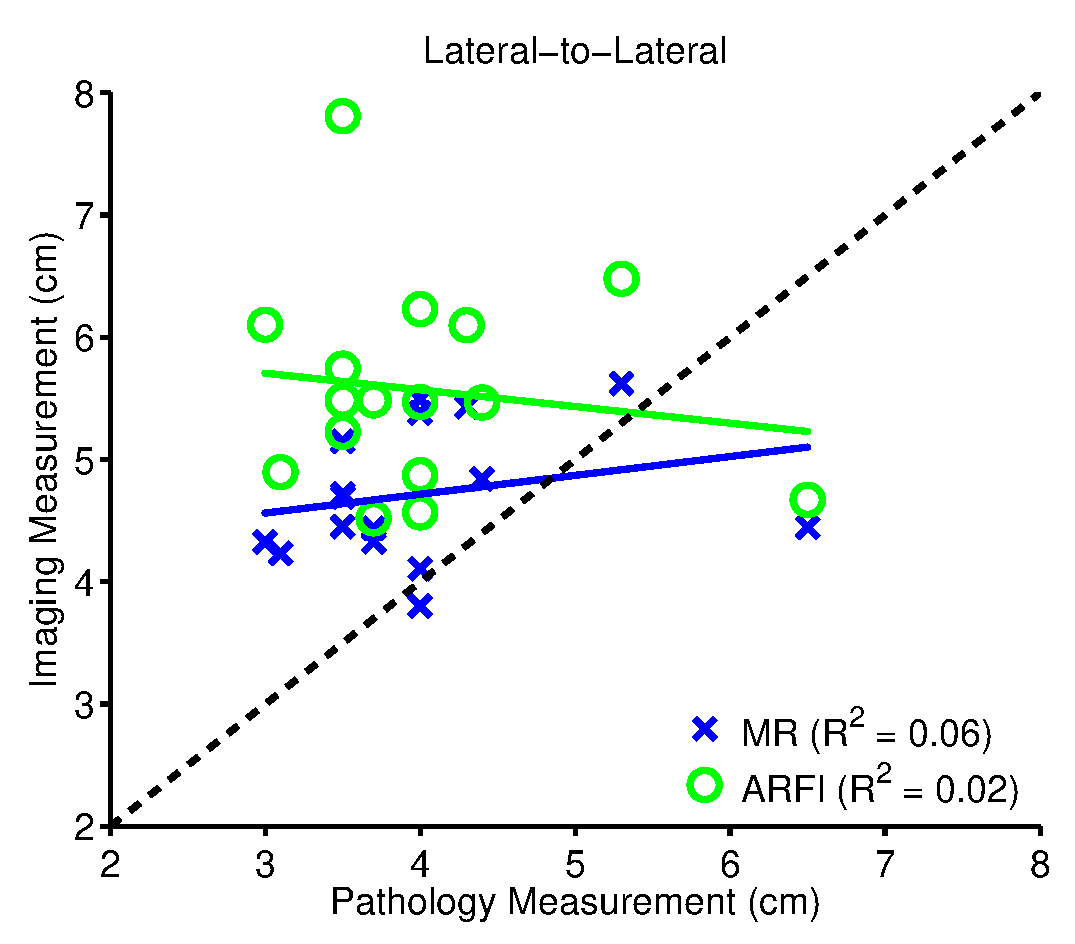
\includegraphics[width=0.3\linewidth]{figs/Lateral-to-Lateral} &
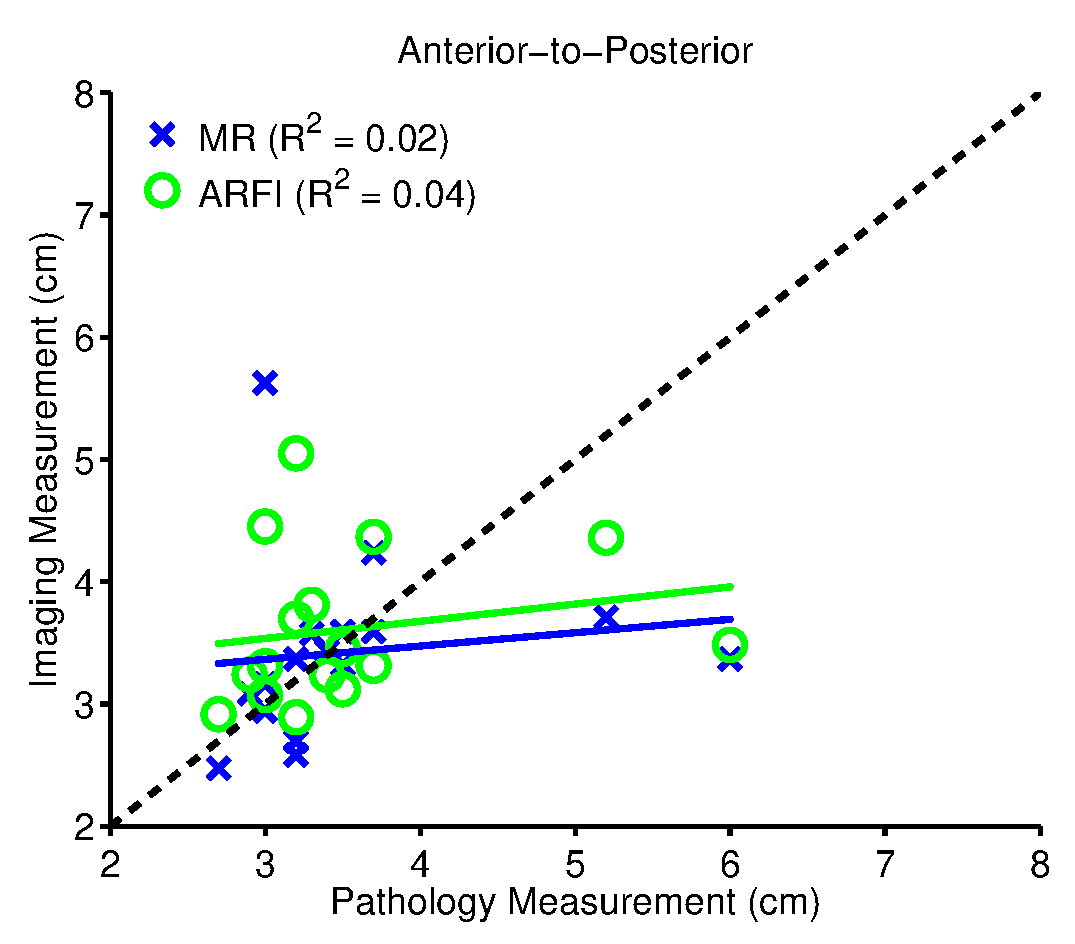
\includegraphics[width=0.3\linewidth]{figs/Anterior-to-Posterior} &
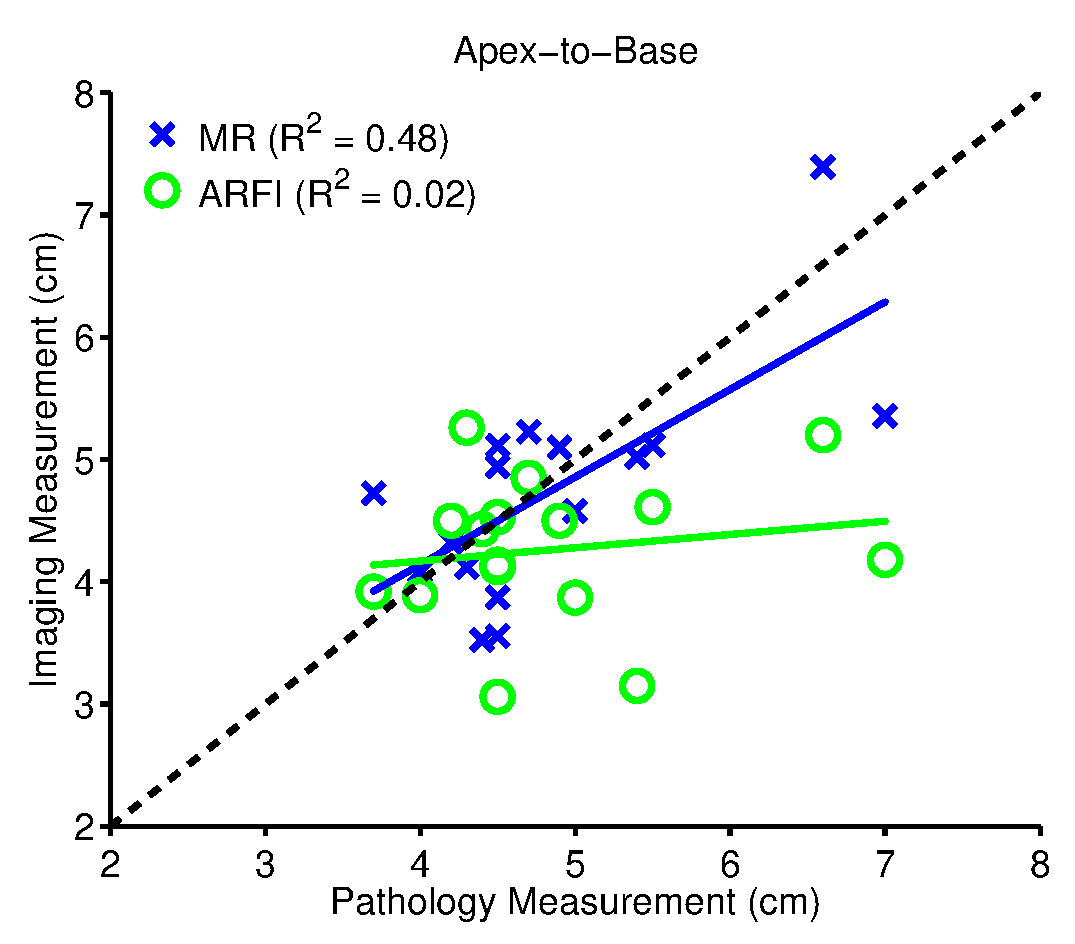
\includegraphics[width=0.3\linewidth]{figs/Apex-to-Base} \\
(a) & (b) & (c) \\
\end{tabular}
\caption{Measurements of the prostate dimensions along the three standard
anatomic axes: lateral-to-lateral (a), anterior-to-posterior (b) and
apex-to-base (c).  The correlation between the imaging axis measurements and
pathology was performed for each orientation.  The black dashed-line represents
the projection of perfectly-correlated measurements between imaging and
patholoy.  Notice that there is no correlation between imaging and pathology in
the lateral-to-lateral and anterior-to-posterior axes, with a general
over-estimation of the lateral-to-lateral axis in the imaging.  The MR
estimation of the apex-to-base dimension showed moderate correlation with
pathology, with the ARFI image apex-to-base approximation having an overall
underestimation in this orientation.  The over-/under-estimation of each imaging modality relative to gross pathology is summarized in Table~\ref{tab:mr_arfi_path_axes}.}
\label{fig:mr_arfi_path_axes} 
\end{figure}


\begin{table}[h!]
\centering
\caption{Difference in ARFI imaging axis measurements relative to MR T2WI measurements.}
\begin{tabular}{|l|l|l|} \hline
 & {\bf ARFI:MR} & {\bf ARFI:MR} \\ 
 & {\bf Total Gland (\%)} & {\bf Central Gland (\%)} \\ \hline 
{\bf Lateral-to-Lateral} & 18.4 $\pm$ 13.9 & 21.5 $\pm$ 14.3 \\ 
{\bf Anterior-to-Posterior} & 7.4 $\pm$ 18 & -0.6 $\pm$ 20.8 \\ 
{\bf Apex-to-Base} & -10.8 $\pm$ 16.8 & -28.8 $\pm$ 9.4 \\ 
\hline
\end{tabular}
\label{tab:mr_arfi_axes_error}
\end{table}


%\begin{figure}[htb!]
\centering
\begin{tabular}{ccc}
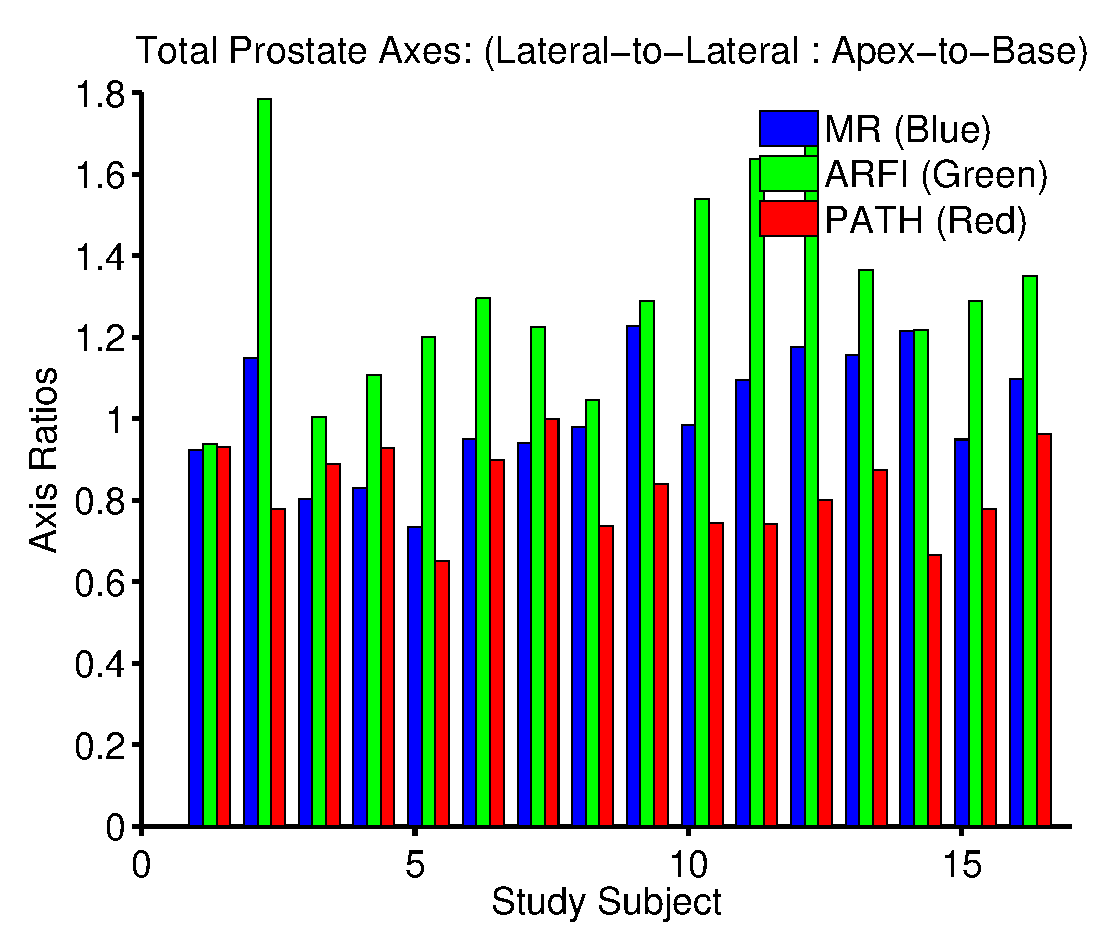
\includegraphics[width=0.3\linewidth]{figs/mr_arfi_total_axes1} &
\includegraphics[width=0.3\linewidth]{figs/mr_arfi_total_axes2} &
\includegraphics[width=0.3\linewidth]{figs/mr_arfi_total_axes3} \\
(a) & (b) & (c) \\
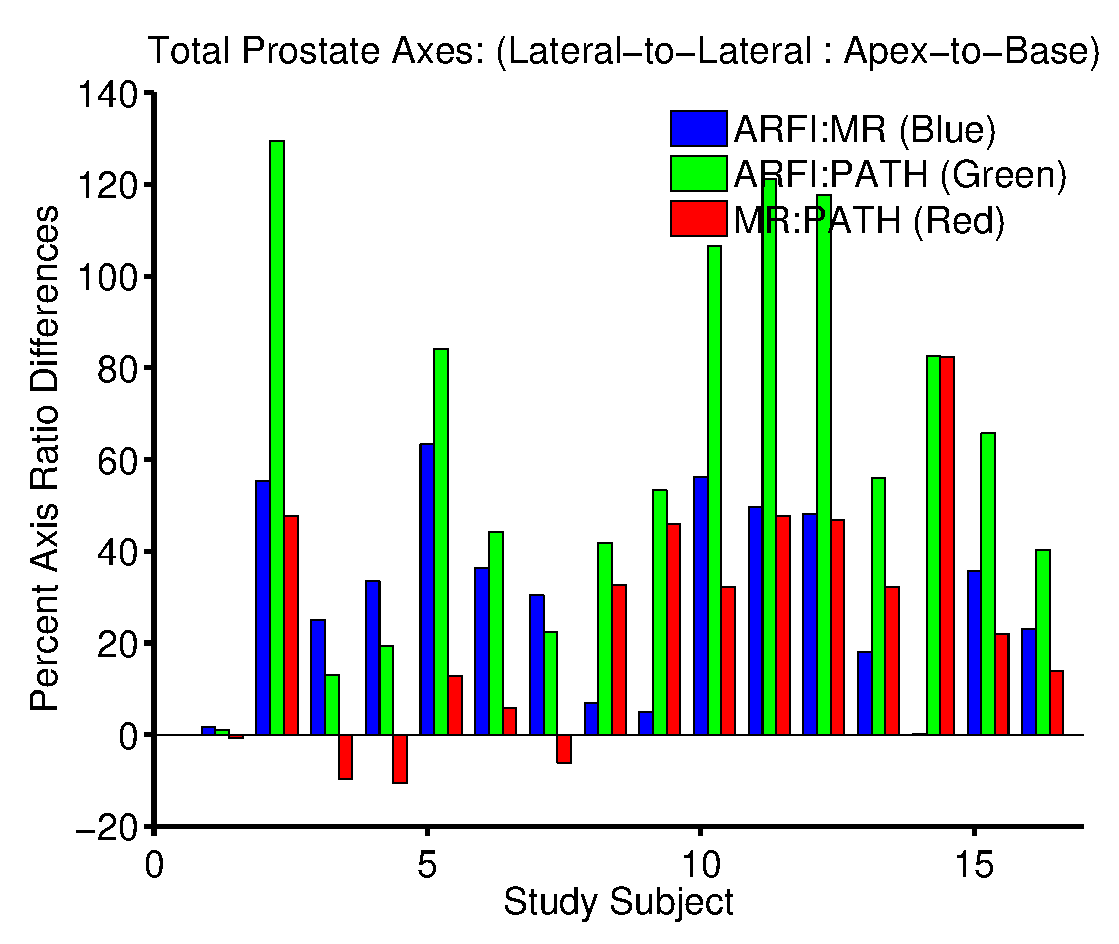
\includegraphics[width=0.3\linewidth]{figs/mr_arfi_total_over_under1} &
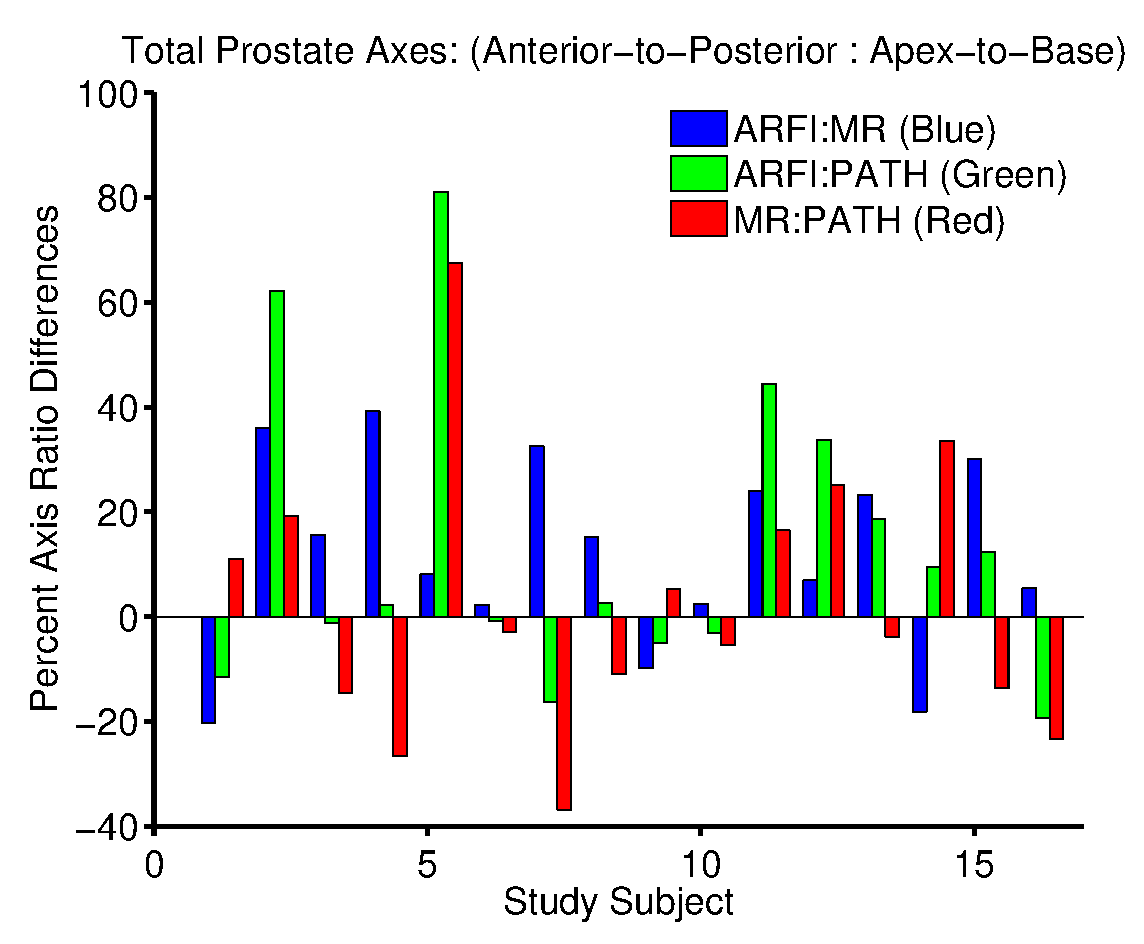
\includegraphics[width=0.3\linewidth]{figs/mr_arfi_total_over_under2} &
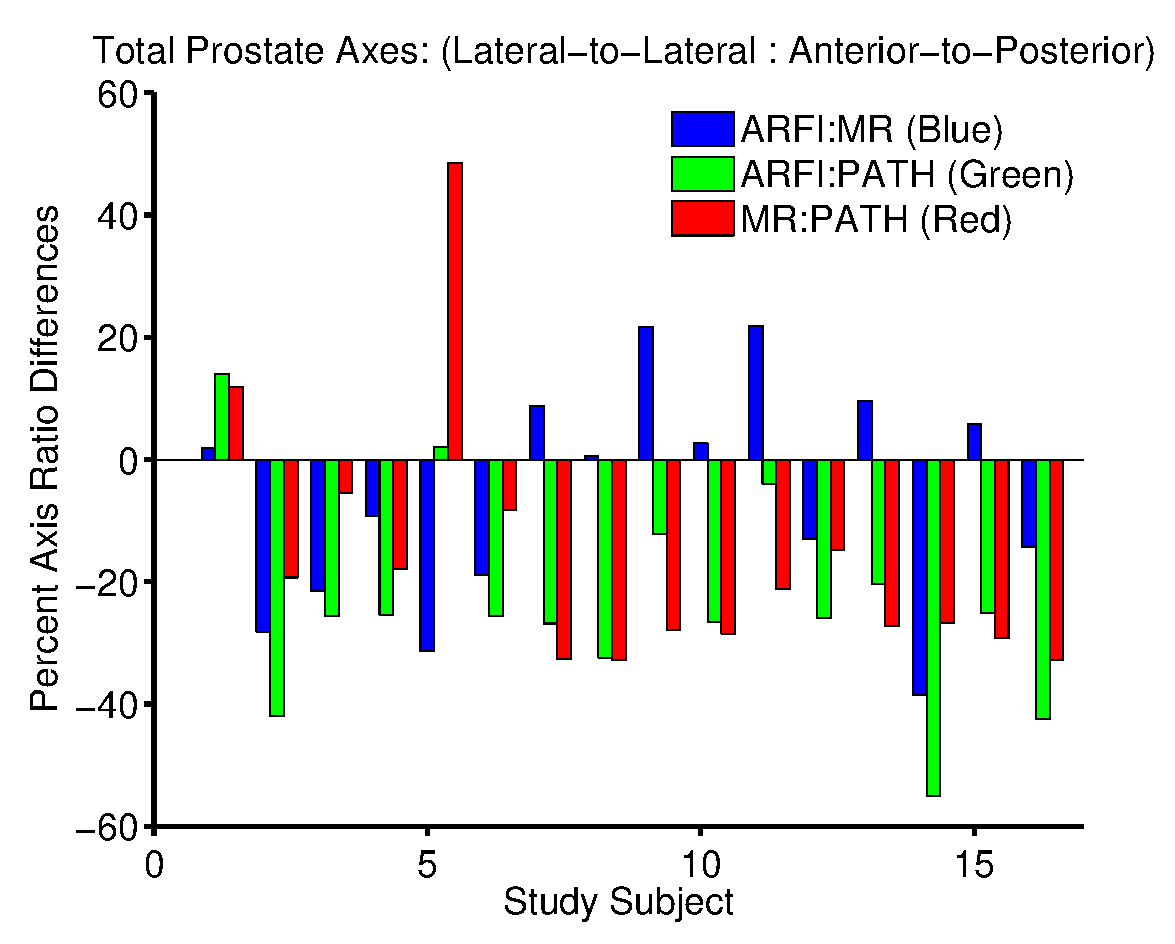
\includegraphics[width=0.3\linewidth]{figs/mr_arfi_total_over_under3} \\
(d) & (e) & (f) \\
\end{tabular}
\caption{Comparison of the ratios of the three anatomic axis measurement ratios
    for T2WI MR (top row, blue), ARFI imaging (top row, green) and gross
    pathology (top row, red).  The over/underestimation of the axis ratios
    between ARFI imaging : T2WI MR : Pathology are shown in the bottom row
    (d-f), with mean ratio differences compiled in
    Table~\ref{tab:axis_ratio_over_under}.}
\label{fig:mr_arfi_total_axes} 
\end{figure}


%\begin{figure}
\centering
\begin{tabular}{ccc}
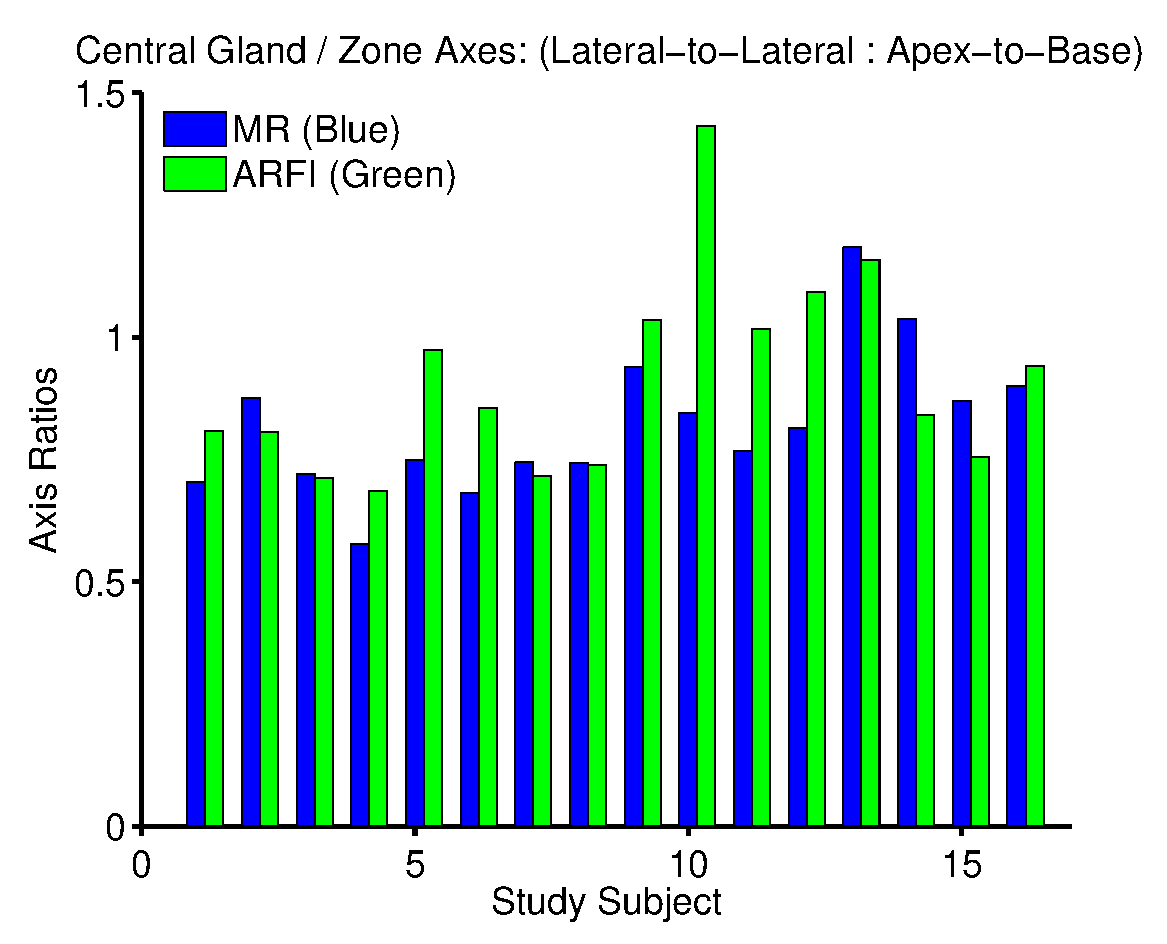
\includegraphics[width=0.3\linewidth]{figs/mr_arfi_central_axes1} &
\includegraphics[width=0.3\linewidth]{figs/mr_arfi_central_axes2} &
\includegraphics[width=0.3\linewidth]{figs/mr_arfi_central_axes3} \\
(a) & (b) & (c) \\
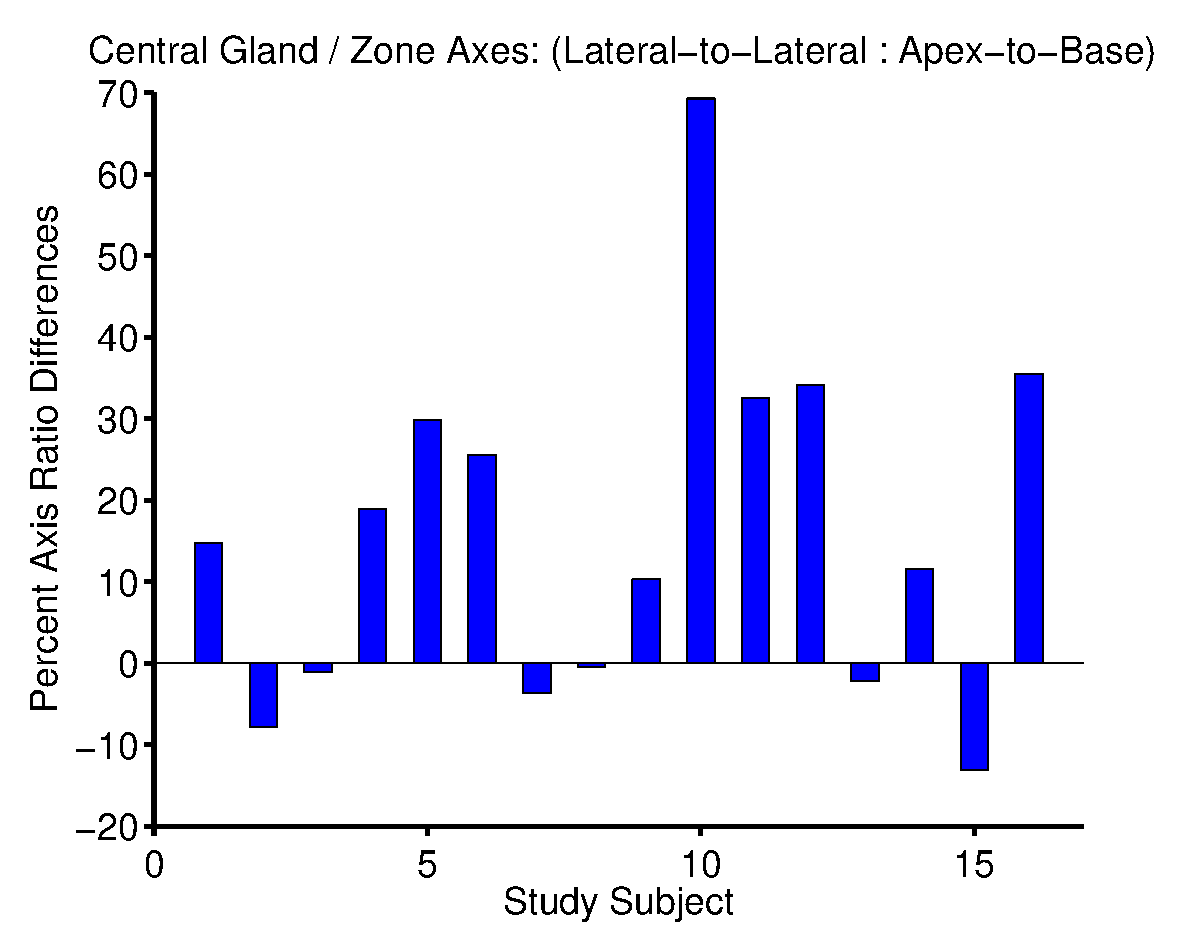
\includegraphics[width=0.3\linewidth]{figs/mr_arfi_central_over_under1.eps} &
\includegraphics[width=0.3\linewidth]{figs/mr_arfi_central_over_under2.eps} &
\includegraphics[width=0.3\linewidth]{figs/mr_arfi_central_over_under3.eps} \\
(a) & (b) & (c) \\
\end{tabular}
\caption{Comparison of the ratios of the three anatomic axis measurement ratios
    for T2WI MR (top row, blue) and ARFI imaging (top row, green).  The
    over/underestimation of the axis ratios between ARFI imaging and T2WI MR
    are shown in the bottom row (d-f), with mean ratio differences compiled in
    Table~\ref{tab:axis_ratio_over_under}.}
\label{fig:mr_arfi_central_axes} 
\end{figure}


%\begin{table}
\centering
\caption{Mean axis ratio differences between ARFI imaging, T2WI MR and
    pathology for the total prostate volume and central gland / zone for the
    imaging modalities.  The three axis ratios analyzed were:
    lateral-to-lateral : apex-to-base (LL:AB), anterior-to-posterior :
    apex-to-base (AP:AB), and lateral-to-lateral : anterior-to-posterior
    (LL:AP).}
\begin{tabular}{|l|l|l|l|l|} \hline
{\bf Image Modality} & {\bf Comparative Measure} & {\bf Total / Central} & {\bf Axes} & {\bf Axis Ratio Difference (\%)} \\ \hline
ARFI & MR & Total & LL:AB & 13.9 $\pm$ 22.9 \\ 
ARFI & PATH & Total & LL:AB & 39.3 $\pm$  27.6 \\ 
MR & PATH & Total & LL:AB & 24.7 $\pm$ 26.0 \\ 
ARFI & MR & Total & AP:AB & 5.2 $\pm$ 22.6 \\ 
ARFI & PATH & Total & AP:AB & 5.4 $\pm$  28.3 \\ 
MR & PATH & Total & AP:AB & 2.5 $\pm$ 26.0 \\ 
ARFI & MR & Total & LL:AP & -6.4 $\pm$ 18.3 \\ 
ARFI & PATH & Total & LL:AP & -23.3 $\pm$  17.1 \\ 
MR & PATH & Total & LL:AP & -16.5 $\pm$ 21.1 \\ 
ARFI & MR & Central & LL:AB & 12.0 $\pm$ 22.5 \\ 
ARFI & MR & Central & AP:AB & -8.8 $\pm$ 20.8 \\ 
ARFI & MR & Central & LL:AP & -15.4 $\pm$ 25.9 \\ 

\hline
\end{tabular}
\label{tab:axis_ratio_over_under}
\end{table}



\section{Discussion}\label{sect:discussion}
This study demonstrated that ARFI imaging delineates zonal anatomy of the
prostate well when compared to MR T2WI, with comparable estimates of total and
central gland volume (Figure~\ref{fig:mr_arfi_volumes}).  Establishing accurate
delineation of the prostate's zonal anatomy is important since PCa has a strong
correlations with location in the prostate, specifically in the peripheral
zone, and accurate capsule delineation will facilitate future efforts to
register 3D imaging datasets between ARFI and MR imaging.  

This was the first quantitative comparison between ARFI imaging and a newly
established clinical imaging modality to evaluate the prostate for PCa
detection and characterization, and we have drawn some useful conclusions in
how our zonal anatomy boundaries are determined during image segmentation.
Poor contrast between the PZ and peri-prostatic fat in B-mode images can lead
to an overestimation of lateral boundaries of the prostate in our ultrasound
datasets compared to MR T2WI, leading to an overall overestimation of prostate
total gland volume.  The anterior aspect of the prostate can also be
challenging to delineate, especially in large prostates, where SNR decreases
with increasing depth away from our rectal wall imaging surface and MR images
suffer from gland heterogeneity in this region~\cite{Gupta2013}, though we had
good agreement between ARFI and MR T2W images in the anterior-to-posterior
dimension (Figure~\ref{fig:mr_arfi_path_axes}(b),
Table~\ref{tab:mr_arfi_axes_error}).  Surprisingly, ARFI imaging consistently
underestimated the extent of the prostate capsule and CG along the apex-to-base
axis relative to MR T2WI (Figure~\ref{fig:mr_arfi_path_axes}(c),
Table~\ref{tab:mr_arfi_axes_error}), though the reasons for this
underestimation are not clear.

This study has several limitations that should be considered when interpreting
these results.  Gross pathology weight and axis measurements could both be
affected by the presence of peri-prostatic tissue that was excised during
radical prostatectomy, especially in cases where more aggressive margins may
have been necessary.  For this reason, unlike the image-to-image measurement
comparisons, all of the image metrics presented relative to pathology metrics
(Figure~\ref{fig:mr_arfi_weight}) were not characterized for absolute accuracy,
but instead, relative correlations were evaluated.  Additionally, the volumes
of the prostate from gross pathologic measurements were approximated as
ellipsoids, which also introduced error, most likely an over-estimation of
volume.  Interestingly, all pathology estimates were thought to have positive
biases, but both imaging modalities tended to overestimate volume relative to the
pathology measurements.

It should also be noted that all of the prostates in this study contained
varying amounts of PCa, BPH and atrophy, all of which can distort the zonal
anatomy, especially in the case of BPH and central gland morphology.  While
younger, healthier prostates could have been targeted, these healthy organs
would not have been excised for pathology characterization, and the zonal
anatomy of a healthy (young) prostate is expected to be different from the
prostate of a middle-age man, who is the target demographic for PCa screening
imaging and PCa characterization. 

This study did not evaluate user biases in image segmentation.  While MR zonal
anatomy delineation has some establishment in the clinical literature, this
study is the first attempt to define the criteria for ARFI imaging zonal
anatomy characteristics, and it is expected that such delineations will
continue to be refined as we acquire more cases and continue to compare with
MRI and pathology data.  Given this limitation, no attempts were made to
further quantify reader-to-reader variability in this work.

Future directions for our research include deeper analysis of our findings,
especially the lateral dimension over-estimation, to improve our anatomic
delineation and assess further its clinical impact.  Technological improvements
to improve anterior prostate boundary delineation in both B-mode and ARFI
imaging are also being pursued and will hopefully allow for the currently
elusive anterior PCa lesions in MR to be seen in ARFI imaging.  3D models of
the prostate and central glands will be used across ARFI and MR imaging
datasets to spatially register them to facilitate correlation of regions of PCa
suspicion between the two modalities, and to correlate with whole-mount
histology of the excised prostate specimens.  This effort will allow the
sensitivity and specificity of each imaging modality for PCa detection and
characterization to be quantified.  While ARFI imaging of the prostate in a
constantly evolving technology, the fact that one can view the different
prostatic zones on ARFI images in addition to MRI is encouraging and could lead
to targeted diagnostic biopsies and therapies with real-time imaging for men
with PCa. 


\section{Conclusions}
The delineation of prostate zonal anatomy in ARFI images has been compared with
the established methods for identifying zonal anatomy using MR T2W images.
Both imaging modalities showed moderate correlations between estimated organ
volume and gross pathologic weights, and ARFI:MR total prostate gland volumes
were well-correlated (R$^2$ = 0.63), but ARFI images yielded prostate volumes
that were, on average, larger (6.1\% $\pm$ 25\%) than MR images, primarily due
to over-estimation of the lateral dimension of the prostate total gland
(\ARFImrTotalLatLatMeanPct~ $\pm$ \ARFImrTotalLatLatStdPct\%), while
over-estimates of the other dimensions were less significant contributors
(\ARFImrTotalAntPostMeanPct~$\pm$ \ARFImrTotalAntPostStdPct\%~and
\ARFImrTotalApexBaseMeanPct~$\pm$ \ARFImrTotalApexBaseStdPct\%).  The central
zone volumes of ARFI and MR images were also moderately correlated (R$^2$ =
0.38), with minimal volume bias between the imaging modalities, but significant
variability case-to-case (-5.0 $\pm$ 39.5\%).  Central zone volume differences
were, again, strongly attributed to over-estimation of the lateral dimension
(\ARFImrCentralLatLatMeanPct~$\pm$ \ARFImrCentralLatLatStdPct\%), with a
significant underestimation of the anterior-to-posterior dimension
(\ARFImrCentralAntPostMeanPct~$\pm$ \ARFImrCentralAntPostStdPct\%).  Strong
variability in central gland volumes is believed to be related to the extent of
benign prostatic hyperplasia (BPH) for select cases.  Overall, ARFI imaging of
the prostate yielded prostate volumes and dimensions that were correlated with
MR T2WI estimates, with biases in the anterior-to-posterior dimension, most
likely related to poor displacement SNR in the anterior region of the prostate
from greater distance from the rectal wall imaging surface, and the lateral
dimension, where contrast between the PZ and peri-prostatic fat could be
limited.  ARFI imaging is a promising low-cost, real-time imaging modality that
can compliment MR imaging for diagnosis, treatment planning and management of
PCa.


\section*{Acknowledgements} 
The authors would like to thank Siemens Medical Solution USA, Ultrasound
Division for their in-kind technical support.  Special thanks to Ned Danieley
for computer system administration support, the pathology assistants in the
Duke University Medical Center for their gross prostate organ processing, and
Matthew Brown for his assistance in designing the optical prostate rotation
feedback system.  This work was supported by NIH R01CA142824 and the Duke
Coulter Translational Grant Program.


\section*{DISCLOSURES}
Some of the authors on this manuscript hold intellectual property related to
ARFI imaging, and commercial licenses of this technology with Duke University
exist.  There are no personal financial disclosures for the authors.


\clearpage
\section{Appendix}\label{sect:appendix}

Tables~\ref{tab:path_data}--\ref{tab:mr_arfi_axes} contain the raw measurements in gross pathology,
MR T2W imaging, and ARFI iamging.

\subsection*{Gross Pathology Measurements}
\begin{table}
\centering
\caption{Pathology Prostate Gross Specimen Metrics}
\begin{tabular}{|l|l|l|l|l|l|} \hline
{\bf Study } & {\bf Weight} & {\bf Lat-Lat} & {\bf Anterior-} & {\bf Apex-Base} & {\bf Ellipsoidal} \\
{\bf Subject} & {\bf (g)} & {\bf (cm)} & {\bf Posterior (cm)} & {\bf (cm)} & {\bf Volume (cm$^3$)} \\ \hline
1 & 37. & 4.3 & 4.0 & 2.9 & 26.10 \\ 
2 & 52. & 4.5 & 3.5 & 3.5 & 28.85 \\ 
3 & 38. & 4.5 & 4.0 & 3.7 & 34.85 \\ 
4 & 84. & 7.0 & 6.5 & 6.0 & 142.87 \\ 
5 & 72. & 6.6 & 4.3 & 3.0 & 44.56 \\ 
6 & 49. & 4.9 & 4.4 & 3.4 & 38.36 \\ 
7 & 25. & 3.7 & 3.7 & 3.2 & 22.93 \\ 
8 & 27. & 4.2 & 3.1 & 2.7 & 18.40 \\ 
9 & 28. & 4.4 & 3.7 & 3.2 & 27.26 \\ 
10 & 42. & 4.7 & 3.5 & 3.2 & 27.55 \\ 
11 & 38. & 5.4 & 4.0 & 3.3 & 37.30 \\ 
12 & 50. & 5.0 & 4.0 & 3.7 & 38.73 \\ 
13 & 29. & 4.0 & 3.5 & 3.0 & 21.98 \\ 
14 & 27. & 4.5 & 3.0 & 3.0 & 21.20 \\ 
15 & 32. & 4.5 & 3.5 & 3.5 & 28.85 \\ 
16 & 62. & 5.5 & 5.3 & 5.2 & 79.33 \\ 

\hline
\end{tabular}
\label{tab:path_data}
\end{table}


\clearpage
\subsection{3D Slicer Segment Model Volume Estimates}
\begin{table}[h!]
\centering
\caption{Comparison of Central Gland / Zone and Total Prostate Volumes in MR T2WI and \textbf{B-mode/}ARFI Imaging}
\begin{tabular}{|l|l|l|l|l|} \hline
{\bf Study Subject} & {\bf MR Central Gland} & {\bf MR Total} & {\bf ARFI Central Gland} & {\bf B-mode Total} \\ 
& {\bf Volume (cm$^3$)} & {\bf Volume (cm$^3$)} & {\bf Volume (cm$^3$)} & {\bf Volume (cm$^3$)} \\ \hline
1 & 12.74 & 24.57 & 14.30 & 19.31 \\ 
2 & 14.26 & 28.51 & 8.37 & 32.90 \\ 
3 & 23.47 & 32.48 & 13.29 & 24.24 \\ 
4 & 17.32 & 32.49 & 10.83 & 28.98 \\ 
5 & 57.56 & 70.95 & 30.37 & 65.55 \\ 
6 & 12.01 & 27.84 & 15.68 & 28.71 \\ 
7 & 8.82 & 19.59 & 11.78 & 23.32 \\ 
8 & 10.97 & 21.28 & 16.02 & 27.72 \\ 
9 & 13.63 & 20.75 & 19.28 & 27.84 \\ 
10 & 23.58 & 36.11 & 33.50 & 58.07 \\ 
11 & 16.57 & 27.33 & 25.22 & 32.78 \\ 
12 & 25.38 & 49.21 & 18.14 & 50.35 \\ 
13 & 9.25 & 26.36 & 6.14 & 32.66 \\ 
14 & 14.79 & 23.36 & 11.60 & 20.68 \\ 
15 & 17.87 & 35.37 & 10.15 & 35.29 \\ 
16 & 33.32 & 48.50 & 19.31 & 31.76 \\ 

\hline
\end{tabular}
\label{tab:mr_arfi_volumes}
\end{table}


\clearpage
\subsection{3D Slicer Segment Model Axis Measurements}
\begin{table}
\centering
\caption{Comparison of Central Gland / Zone and Total Prostate Major / Minos Axes in MR T2WI and ARFI Imaging}
\begin{tabular}{|l|l|l|l|l|l|l|l|l|l|l|l|l|} \hline
{\bf Study} & {\bf MR} & {\bf MR} & {\bf MR} & {\bf MR} & {\bf MR} & {\bf MR} & {\bf ARFI} & {\bf ARFI} & {\bf ARFI} & {\bf ARFI} & {\bf ARFI} & {\bf ARFI} \\ 
{\bf Subject} & {\bf CA} & {\bf CL} & {\bf CE} & {\bf TA} & {\bf TL} & {\bf TE} & {\bf CA} & {\bf CL} & {\bf CE} & {\bf TA} & {\bf TL} & {\bf TE} \\
 & {\bf (cm)} & {\bf (cm)} & {\bf (cm)} & {\bf (cm)} & {\bf (cm)} & {\bf (cm)} & {\bf (cm)} & {\bf (cm)} & {\bf (cm)} & {\bf (cm)} & {\bf (cm)} & {\bf (cm)} \\ \hline
1 & 4.12 & 2.90 & 2.45 & 4.12 & 3.80 & 3.09 & 4.34 & 3.51 & 2.28 & 5.26 & 4.94 & 3.14 \\ 
2 & 3.87 & 3.39 & 2.80 & 3.87 & 4.45 & 3.59 & 4.03 & 3.25 & 1.66 & 3.06 & 5.46 & 3.86 \\ 
3 & 4.82 & 3.48 & 3.27 & 5.11 & 4.11 & 3.59 & 4.53 & 3.23 & 2.29 & 4.53 & 4.55 & 3.68 \\ 
4 & 5.35 & 3.08 & 2.87 & 5.36 & 4.45 & 3.37 & 3.82 & 2.62 & 2.35 & 4.18 & 4.63 & 3.66 \\ 
5 & 6.22 & 4.66 & 4.98 & 7.39 & 5.43 & 5.63 & 5.20 & 5.06 & 2.42 & 5.20 & 6.24 & 4.28 \\ 
6 & 5.05 & 3.44 & 3.44 & 5.10 & 4.84 & 3.44 & 4.63 & 3.96 & 2.29 & 4.50 & 5.83 & 3.10 \\ 
7 & 4.47 & 3.33 & 2.26 & 4.72 & 4.44 & 2.58 & 4.77 & 3.42 & 2.40 & 3.92 & 4.80 & 2.84 \\ 
8 & 4.30 & 3.20 & 2.10 & 4.32 & 4.23 & 2.48 & 5.72 & 4.23 & 2.52 & 4.50 & 4.71 & 2.97 \\ 
9 & 3.52 & 3.31 & 2.19 & 3.52 & 4.33 & 2.70 & 4.73 & 4.90 & 2.69 & 4.43 & 5.71 & 3.06 \\ 
10 & 5.24 & 4.43 & 2.69 & 5.23 & 5.15 & 3.37 & 5.02 & 7.19 & 2.20 & 4.85 & 7.46 & 3.20 \\ 
11 & 5.02 & 3.85 & 2.73 & 5.02 & 5.50 & 3.57 & 4.24 & 4.31 & 2.72 & 3.15 & 5.16 & 2.78 \\ 
12 & 4.55 & 3.70 & 3.30 & 4.58 & 5.38 & 4.24 & 4.24 & 4.63 & 2.34 & 3.87 & 6.74 & 3.83 \\ 
13 & 3.40 & 4.03 & 2.01 & 4.08 & 4.72 & 2.94 & 2.84 & 3.29 & 1.91 & 3.89 & 5.31 & 3.46 \\ 
14 & 3.56 & 3.69 & 2.54 & 3.56 & 4.33 & 3.17 & 4.18 & 4.84 & 2.29 & 4.14 & 5.04 & 3.02 \\ 
15 & 4.79 & 4.17 & 2.56 & 4.95 & 4.69 & 3.32 & 5.00 & 3.78 & 3.08 & 4.12 & 5.31 & 3.60 \\ 
16 & 5.11 & 4.60 & 3.11 & 5.12 & 5.62 & 3.71 & 5.03 & 6.14 & 3.13 & 4.61 & 6.23 & 3.52 \\ 

\hline
\end{tabular}
\label{tab:mr_arfi_axes}
\end{table}



\clearpage
\bibliographystyle{IEEEtran}
\bibliography{library}

\end{document}
